%% PNAStwoS.tex
%% Sample file to use for PNAS articles prepared in LaTeX
%% For two column PNAS articles
%% Version1: Apr 15, 2008
%% Version2: Oct 04, 2013

%% BASIC CLASS FILE
\documentclass{pnastwo}

%% ADDITIONAL OPTIONAL STYLE FILES Font specification

%\usepackage{pnastwoF}
%\usepackage{cite}
\usepackage[numbers,round,sort,compress]{natbib}
\bibpunct{(}{)}{,}{n}{,}{,}  % https://xianblog.wordpress.com/tag/natbib/ (allows natbib with PNAS)
\usepackage{lineno}
\setlength\linenumbersep{2pt}
\usepackage{placeins}
\usepackage{float}
%\usepackage{subfigure}
\usepackage{wrapfig}
%\setlength\belowcaptionskip{-2cm}
%\setlength{\textfloatsep}{5pt plus 1.0pt minus 2.0pt}

%% OPTIONAL MACRO DEFINITIONS
\def\s{\sigma}
%%%%%%%%%%%%
%% For PNAS Only:
\url{www.pnas.org/cgi/doi/10.1073/pnas.0709640104}
\copyrightyear{2008}
\issuedate{Issue Date}
\volume{Volume}
\issuenumber{Issue Number}
%\setcounter{page}{2687} %Set page number here if desired
%%%%%%%%%%%%

\begin{document}

\title{A Full Accounting of Landcover Map Error and Bias and Their Impacts on Assessments of Global Change}
%\title{Our Understanding of Global Change is Built on a Shaky Foundation}

\author{Lyndon Estes\affil{1}{Princeton University, Princeton, NJ USA},
Peng Chen\affil{2}{Indiana University, Bloomington, IN USA},
Stephanie Debats\affil{1}{Princeton University, Princeton, NJ USA},
Tom Evans\affil{2}{Indiana University, Bloomington, IN USA},
Fanie Ferreira\affil{3}{GeoTerraImage, Pretoria, RSA},
Gabrielle Ragazzo\affil{1}{Princeton University, Princeton, NJ USA},
Justin Sheffield\affil{1}{Princeton University, Princeton, NJ USA}
Adam Wolf\affil{1}{Princeton University, Princeton, NJ USA}
\and
Kelly Caylor\affil{1}{Princeton University, Princeton, NJ USA}}

\contributor{Submitted to Proceedings of the National Academy of Sciences
of the United States of America}

%%%Newly updated.
%%% If significance statement need, then can use the below command otherwise just delete it.
%\significancetext{LDE developed the concept of the study, conducted the analysis, data interpretation and drafted the manuscript. \color{red}{To be completed}}

\maketitle

\begin{article}
\begin{abstract}
{Blah blah.}
\end{abstract}

\keywords{landcover | bias | remote sensing | agriculture | crop yield | harvested area | carbon | agent-based model | landscape}

\abbreviations{GTI, GeoTerraImage; SSA, sub-Saharan Africa}
\linenumbers

\dropcap{T}he nature and distribution of landcover provides significant insight into econonomic processes \cite{lambin_modelling_1997} because human endeavors are so closely tied to how we transform land, whether it be the felling of ancient forests for farmland or converting that farmland into office parks. The vastness of our alteration of Earth�s landscapes suggests that landcover is a prime mediator of many environmental and social processes that drive or are affected by global change \cite{lambin_modelling_1997}, such as agricultural production and food security \cite{lark_cropland_2015,wright_recent_2013, licker_mind_2010}, carbon cycling \cite{asner_high-resolution_2010,gaveau_major_2014}, biodiversity loss \cite{newbold_global_2015,luoto_predicting_2004}, and changes in human demography \cite{linard_assessing_2010}. Like any view into nature, resolution and fidelity at fine scales are the keys to unlocking more granular and mechanistic insights into these processes \cite{see_improved_2015}. It is therefore unsurprising to see the explosive growth in private sector initiatives to develop new Earth observing capabilities, which range from small hobbyist drones\footnote{e.g. 3DRobotics, DJIA} to satellite arrays\footnote{Planet Labs, Skybox}, in order to add value to industries such as agriculture, mining, and construction. This rapid growth in fine-scale landcover mapping capability is creating new opportunities to develop actionable information for traditionally public-sector concerns, such as agricultural development\footnote{USAID's Feed the Future}, drought and flood adaptation\footnote{Global Index Insurance Facility, www.indexinsuranceforum.org}, and carbon cycle management\footnote{United Nations REDD+, www.un-redd.org/aboutredd}. But while the demand for more nuanced, landcover-based insights is growing, there is only now the opportunity to use finer-scaled imagery to comprehensively interrogate the accuracy and biases in the landcover products that have become ubiquitous in global change research.

Global landcover data can only practically be derived from satellite imaging, but in many regions the cover types of interest are smaller, on average, than the sensor resolution, or spectrally indistinct from other neighboring covers, and these factors propagate classification errors \cite{see_improved_2015,lobell_use_2013,estes_diylandcover:_2015}. The result is that landcover maps are generally inaccurate at finer scales and disagree substantially with one another, particularly in those parts of the world undergoing the most rapid land use changes \cite{estes_projected_2013,fritz_comparison_2010,fritz_cropland_2011}.  

Errors in landcover products are widely-acknowledged \cite{fritz_comparison_2010, fritz_cropland_2011, see_improved_2015, fritz_mapping_2015,verburg_challenges_2011}, and there are a variety of efforts underway to improve landcover maps, particularly for agriculture \cite{fritz_geo-wiki:_2012,estes_diylandcover:_2015}. What is less known is the degree to which these errors bias analyses derived from the distributional and areal information in landcover. Errors are hard to quantify because spatially extensive reference data are not available for most regions of the world--particularly over Africa and other developing regions. Error assessments therefore typically rely on a small number of ground truth points for a bottom-up assessment or aggregated survey data for a top-down sanity check. For this reason, we have a better understanding of discrepancies between landcover datasets in relation to country-level statistics \cite{fritz_comparison_2010,fritz_cropland_2011,kaptue_tchuente_comparison_2011}, which offers little direction for how to arrive at a true number. 

Being unable to fully quantify the errors in landcover maps of course makes it difficult, if not impossible, to quantify their impact on downstream analyses. There has been some work examining how such error influences climate simulations \cite{ge_impacts_2007}, agricultural land use patterns \cite{schmit_limitations_2006}, and carbon flux \cite{quaife_impact_2008} and human population estimates \cite{linard_assessing_2010}, but these either use simulated landcover errors \cite{ge_impacts_2007} or compare relevant differences in estimates between different satellite-derived landcover maps \cite{linard_assessing_2010, quaife_impact_2008}. One exception is a Belgian study  \cite{schmit_limitations_2006} that used ground-collected farm parcel data to assess how landcover map errors bias measurements of agricultural land use patterns, but the study extent was fairly small and the validation data were discontiguous. 

Just as a building needs a solid foundation, global change science needs to be based on sound landcover data. There is thus an urgent need to more precisely quantify landcover map errors and how these vary over large regions, particularly for the regions where landcover is changing most rapidly yet is most poorly known.  We address this need here, using a unique, high accuracy agricultural landcover map for the entire country of South Africa to conduct a spatially comprehensive, bottom-up quantification of error in several latest generation landcover maps that are widely used in global change studies. We use these errors to assess the biases and accuracies of i) these landcover data, ii) how landcover properties influence map errors, iii) how bias and accuracy change with aggregation scale, with the specific goal of determining ``safe'' scales for drawing area-based inferences, and iv) how landcover error propagates through ``downstream'' analyses that represent several major global change research areas, including biogeochemical and land use change studies, food security assessments, land surface hydrology and climatology, and human geography.  

\vspace{-0.5 cm}
\section{Study area and landcover data}
South Africa comprises nearly 6\% of sub-Saharan Africa's (SSA) landmass, and has a large, diverse agricultural sector, ranging from large commercial operations to smallholder farms \cite{hardy_rainfed_2011,estes_using_2014}. This diversity suggests that the country's agricultural landcover spans the range of types that are found throughout the rest of SSA.  

The South African government commissioned a whole-country cropland boundary map to enhance its annual collection of agricultural statistics \cite{fourie_better_2009}. The map was made by trained workers who visually interpreted high resolution satellite imagery ($<$5 m SPOT imagery) and manually digitized field boundaries following a standardized mapping protocol. The resulting vectorized field maps, provide a unique, high quality reference dataset describing South African crop field distributions and size classes for the period 2009-2011, and are 97\% accurate in distinguishing cropland from non-cropland at 200 m resolution. We intersected the field vectors with a 1 km grid, and calculated the percent of each cell occupied by fields to create a gridded cropland reference map. 

We compared the reference map with similar maps derived from four existing landcover datasets. We obtained South Africa's 30 m resolution National Landcover map (SA-LC) for 2009 \cite{sanbi_national_2009}, the 500 m resolution MODIS Landcover for 2011 \cite{land_processes_distributed_active_archive_center_lp_daac_modis_2011, friedl_modis_2010}, the 300 m resolution GlobCover 2009 \cite{arino_global_2012}, and the new 1 km Geo-wiki hybrid-fusion cropland map for Africa \cite{fritz_mapping_2015}. We chose these particular datasets because they are nearly contemporaneous with our reference data, and represent the major types of landcover products used by researchers: SA-LC typifies the higher resolution, Landsat-derived maps that are developed individually for many countries \cite[e.g.][]{fry_completion_2009}, MODIS and GlobCover are widely used global-scale products \cite{gross_monitoring_2013, shackelford_conservation_2015}, while Geo-Wiki incorporates the first three datasets and represents the current state-of-the-art in landcover mapping. We extracted the cropland classes from the first three datasets and converted these to 1 km resolution percent cropland estimates, resulting in 4 maps (hereafter simply the ``cropland maps'') to compare to our reference map.  

\vspace{-0.5 cm}
\section{Quantifying Error and Bias}
We first calculated errors in pixel-wise estimated cropland percentages by differencing the reference map with each cropland map at each of the five aggregation scales (1-100 km). We used these errors to calculate map bias (the mean pixel-wise error) and accuracy (the mean absolute error, and how these vary with scale. Next, we assessed the degree to which the average cropland cover in agricultural landscapes, a descriptor of landcover pattern, impacts map accuracy.    

To investigate how landcover map error can impact downstream global change research, we quantified the biases and accuracies in five landcover-based analyses built upon our reference and cropland maps. The first three represented ``first-order'' analyses, in which a variable of interest is mapped onto a landcover type(s) using a simple empirical relationship. The first of these was the widely used International Panel on Climate Change's Tier-1 approach for mapping vegetative carbon stocks, as developed by \cite{ruesch_new_2008}. The second was maize yield maps derived by disaggregating district-scale agricultural census data for both maize yield and harvested area \cite[following][]{monfreda_farming_2008,ramankutty_farming_2008}, from which we calculated the third map, gridded maize production estimates. Maps based on these analyses underpin many assessments of crop productivity and production \cite[e.g.][]{foley_solutions_2011,licker_mind_2010}.  

The other two analyses can be considered second-order, wherein a process model draws on the cover types' values to calculate an output value. For the first of these, we used the Variable Infiltration Capacity \cite{liang_simple_1994} land surface hydrology model to calculate monthly evapotranspiration, using the reference and cropland maps to adjust landcover-specific leaf area index (LAI) values that VIC uses to partition water vapor fluxes into their evaporative and transpirative components. In the second example, we examined how these map errors impact the land allocation process of an agent-based food security model \cite{chen_dependency_2013}. 

\vspace{-0.5 cm}
\section{Landcover maps}
\subsection{Bias and accuracy}

We created the 1 km reference map after removing all field types classified as communal/smallholder agriculture (individual fields in this category were not delineated, thus they were removed to prevent potential cropland area overestimates, SI) or permanent tree-crops (SI), and calculated the total cropland extent in the remaining area (1,081,000 km$^2$, or 90\% of South Africa). The 2011 reference map showed a cropland area of 104,304 km$^2$, which the SA-LC and GeoWiki maps overestimated by 31 and 10\%, respectively, and GlobCover and MODIS underestimated by 18 and 23\%.  

We then aggregated the reference and each cropland map to 5, 10, 25, 50, and 100 km resolutions, and subtracted the four landcover maps from each reference (2007 and 2011) map at each scale of aggregation to assess error patterns (Fig. 1A). Negative pixels here represent overestimation error, while positive values indicate underestimates.

%\vspace{-0.5 cm}
\begin{figure*}[ht]
%\begin{wrapfigure}{c}{1\textwidth}
\centerline{\includegraphics[width=0.99\textwidth]{figures/figure1.pdf}}
\caption{(A) Errors in the percent cropland estimates resulting from each of the four cropland maps relative to the reference map at different scale of pixel aggegation. Rows indicate the landcover map being assessed (by subtraction from the reference map), while columns refer to resolution of aggregation. White indicates areas with no data where communal farmlands or plantation forests were removed from analysis. (B) The bias (mean error) and accuracy (mean absolute error [MAE]) of each cropland map at each scale of aggregation. Bias estimates (represented by symbols) fall within the semi-transparent bars, mean absolute errors in the solid bars, with bar colors coded to specific cropland maps. The symbols indicate the method of calculating each metric, either by averaging across the entire country, within the union of  agricultural areas (cropland $>$0.05\%) for each reference-cropland map combination, or as the average of the averages calculated per 5\% bin of cropland cover, a measure of error that is independent of cropland density.}\label{afoto}
\end{figure*}
%\end{wrapfigure}


%\begin{figure*}[htp]
%\centering
%    \subfigure[random caption 1]{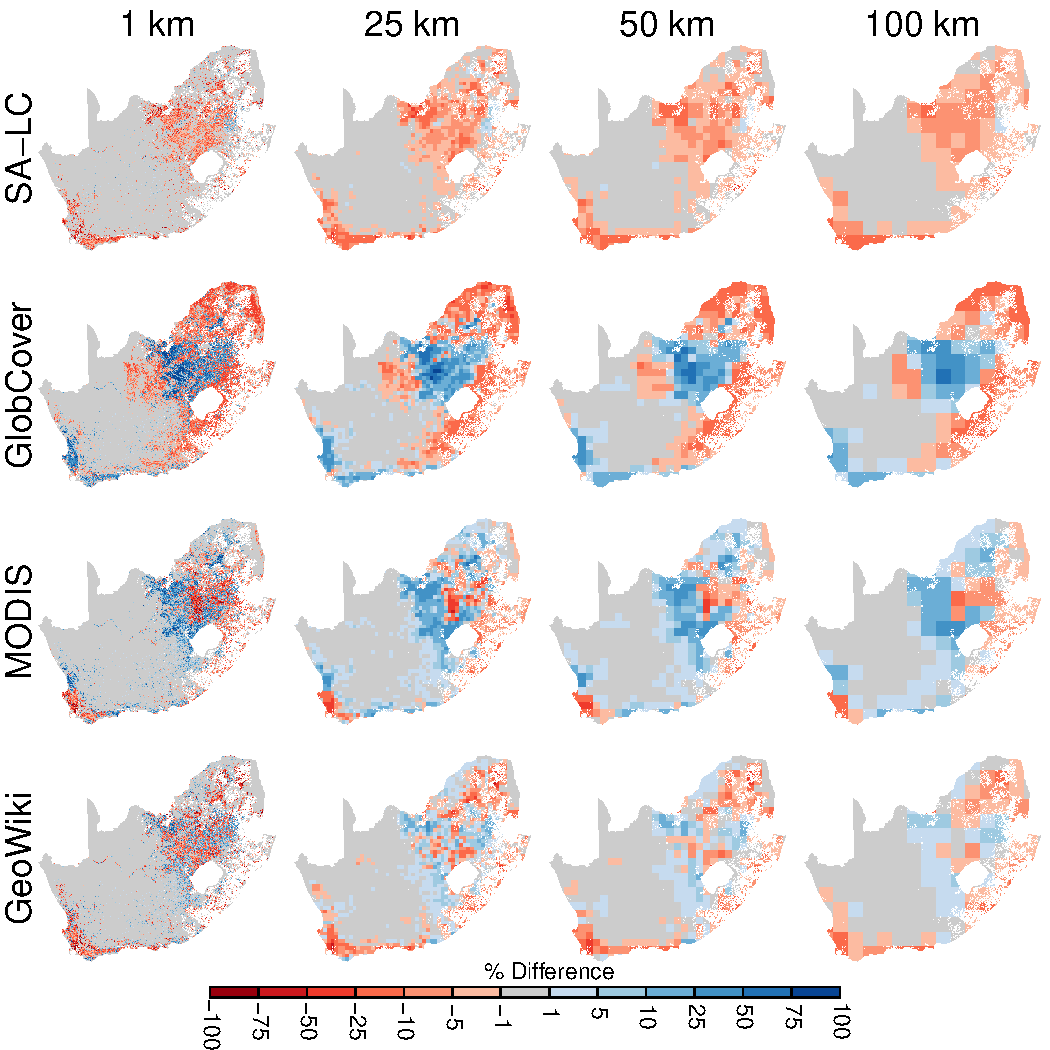
\includegraphics[scale=0.49]{figures/bias_map.pdf}}\quad
%     \subfigure[random caption 1]{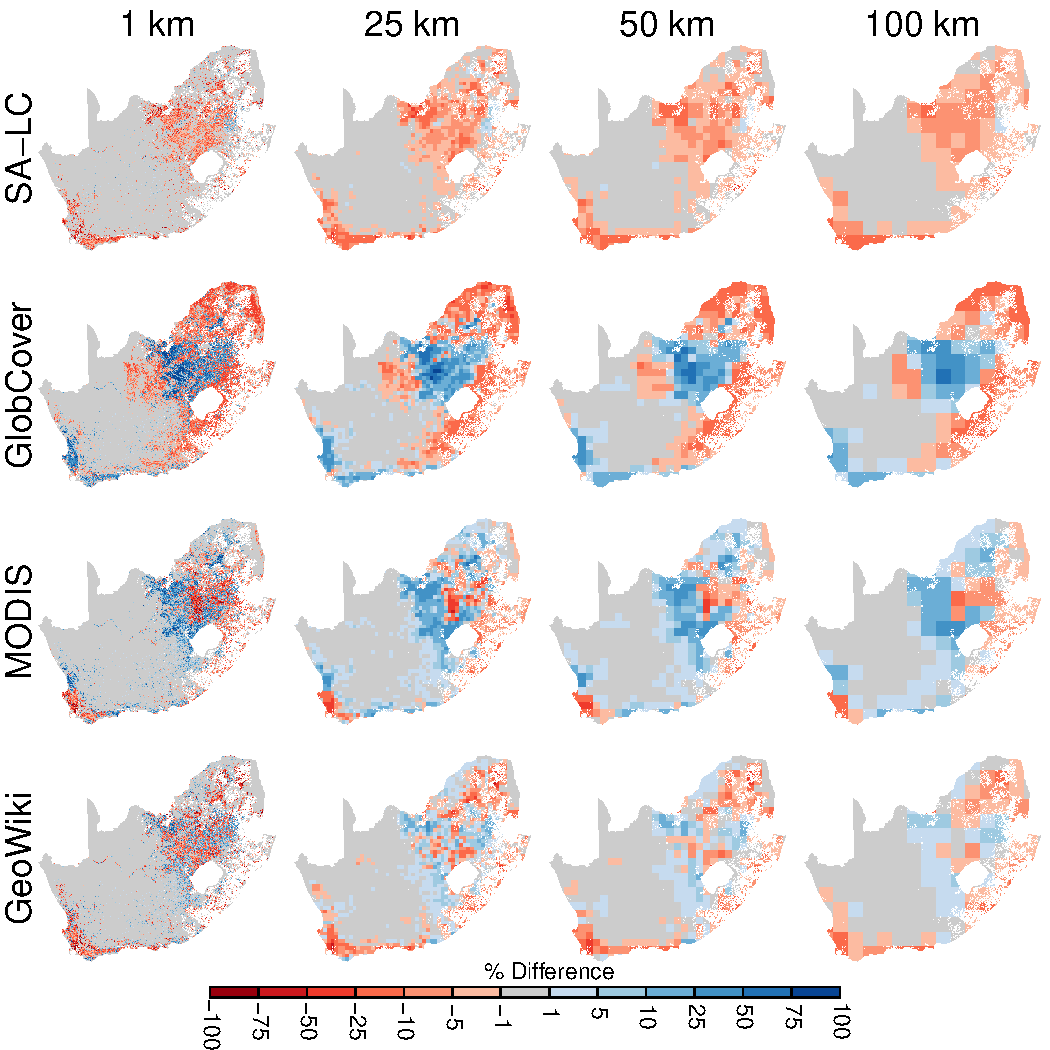
\includegraphics[scale=0.49]{figures/bias_map.pdf}}
%\end{figure*}

\linenumbers
The most pronounced errors were in the MODIS and GlobCover maps, which both underestimated cropland extent by 10-75\% in the center of the country (blue areas in Fig. 1A, and the dominant production region), and overestimated along the eastern to northern margins (red areas in Fig. 1A). All maps have less than +/-5\% bias (crosses in semi-transparent bars, Fig. 1B), at all aggregation scales, when errors are averaged across the entire country, due to the extensive non-agricultural areas in the country that were effectively discerned by all maps. The whole country mean absolute error (the measure of map accuracy) were a few percent higher values in most cases, but still $<$10\%, except for GlobCover ($\sim$11\%) at 1 km resolution. Biases increase only slightly when errors are averaged within the combined agricultural regions (areas with greater than 0.05\% cropland, indicated by circles in transparent bars in Fig. 1B) of the reference and each cropland map, but accuracy decreases substantially, with mean absolute errors increasing to 10\% for SA-LC and around 20\% for MODIS, GlobCover, and GeoWiki at 1 km resolution (circles in solid bars in Fig. 1B), and remain between 5-10\% for all three datasets even at 25 km of aggregation. 

As a third measure, we calculated bias and mean absolute error by averaging their mean per-ventile values (i.e. the average bias or accuracy value for areas have 0-5\% cropland, 5-10\% cropland, etc.). These provide density independent measures of map performance because they remove the dominance any particular level of cover has on map accuracy, which in this case was the 0-5\% cover class where map performance was best (SI). Calculated this way, bias and accuracy were substantially worse. The average bias jumped to 21\% for MODIS and 34\% for GlobCover at 1 km resolution (Fig. 1B), meaning that each map had a strong tendency to underestimate cropland. This decreased with pixel aggregation, falling to 8\% at 50 km for MODIS, but remaining as high as 14\% at 100 km for GlobCover. SA-LC bias was smaller in magnitude, but tended towards cropland overestimates of 5-10\% at all aggregation scales. GeoWiki alone was relatively unbiased, but showed substantial inaccuracy with a density-independent mean absolute error of 23\%, which dropped below 10\% only above 25 km of aggregation. GlobCover was by far the most inaccurate, having $>$35\% mean absolute error at 1 km and 17\% at 100 km, following by MODIS (over 30\% at 1 km and 11\% at 100 km). SA-LC was the most accurate of all four maps with the density-independent measure, ranging from just above 10\% mean absolute error at 1 km to 5\% at 100 km. 

\subsection{Landscape characteristics and error}
The density-independent measures indicate that error and bias increase with cropland density, which suggests that map error varies as a function of the typical abundance of cover in the landscape being imaged. To investigate the relationship between cover density and map accuracy, we calculated the mean density for agricultural pixels ($>$0.05\% cropland) in the 1 km reference map within the boundaries of 354 magisterial districts (South Africa's finest administrative unit, averaging 3,445 km$^2$; SI Figure S3), providing a landscape-scale measure representing typical cropland density. We then extracted the cropland map errors for these same pixels, and calculated their district-wise mean absolute errors. 

A generalized additive model fit to district-level mean absolute error (log-transformed) shows that error peaks at 50-60\% cropland cover for all but the GlobCover map (which continued to increase with cropland cover), and is lowest when the landscape is dominated either by cropland or other cover types (Fig. 2). In other words, accuracy is generally lowest when cropland cover is mixed evenly with other cover types. GlobCover's accuracy continued to decrease with cropland density because the dominant cover class contributing to the percentage cropland estimate was a mixed class defined as 50-70\% crops mingled with other vegetation, thus the maximum percentage was constrained by this mixture range.  

%\vspace{-1 cm}
\begin{figure}[ht]
\centerline{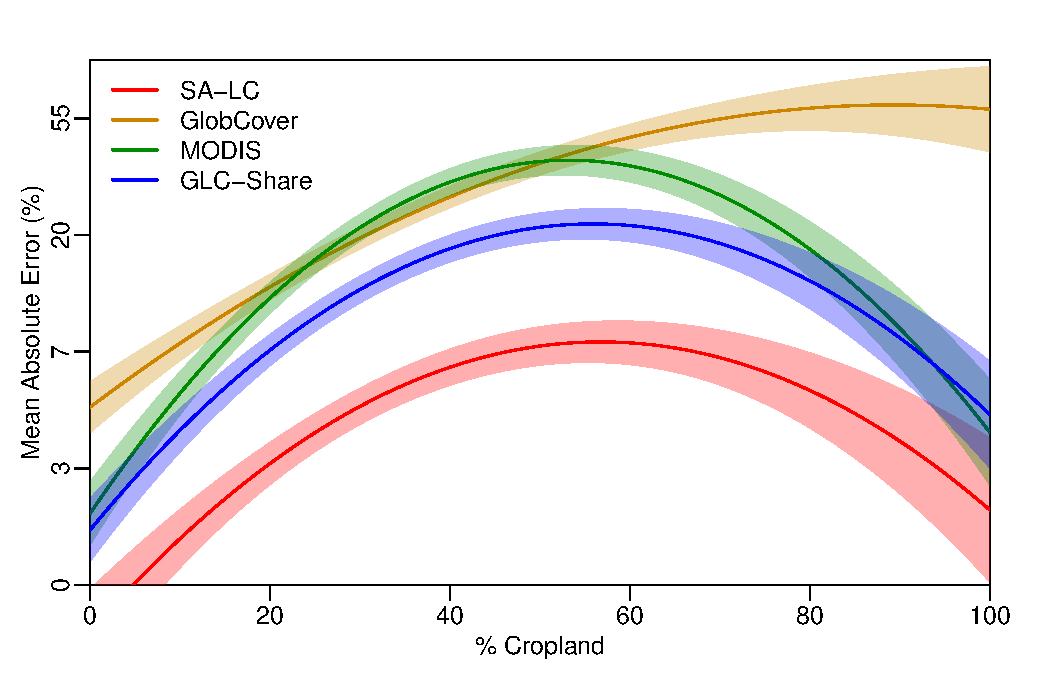
\includegraphics[width=.5\textwidth]{figures/biases_md_lnorm_gam_mu0.pdf}}
\caption{The relationship between map accuracy (the mean absolute error) in cropland maps and the actual cropland cover within agricultural landscapes (reference map pixels having $>$0.5\% cropland), here defined by the boundaries of magisterial districts (n = 345), as fit with a generalized additive model. Prediction curves are color-coded to the different cropland maps, with the solid line indicating predicted absolute bias, and the lighter shading the standard error of the coefficients.}
\label{afoto}
\end{figure}

\section{First-order analyses}
\subsection{Tier-1 carbon estimates}
Using the methods provided by \cite{ruesch_new_2008}, we calculated average carbon densities for African forests, secondary forests, shrublands, croplands, grasslands, and sparse habitats (semi-arid grasslands and low shrublands), and assigned cropland carbon values to map cells in proportion to their cropland cover. For the non-cropland proportions, we assigned the carbon value from each of the other types, creating five different carbon maps for each landcover map at each aggregation scale (Fig. S4), which allowed us to test how carbon estimates vary as a function of i) cropland map bias and ii) the characteristics of adjacent cover types. 

The difference between total carbon stocks for the country made using any of the cropland maps were within +/-3\% of those based on the reference map, regardless of which cover type was adjacent to cropland (Table S1), because the large of non-cropland in the country ($\sim$50-70\%, Fig. 1) dilutes any map errors. Comparing total stocks between maps for just the agricultural area (30-50\% of the country) reveals much greater differences (Table S1). SA-LC overestimated carbon stocks by just 2\% when the adjacent cover type was forest, and up to 15\% when it was sparse cover. MODIS ranged from negligible differences in denser carbon classes (forest, secondary forest, and shrublands) to 8-13\% underestimates for the grassland and sparse classes. GeoWiki underestimated for all types, from $<$1\% for sparse cover to 8\% for forest. GlobCover grossly overestimated total carbon stocks for agricultural areas, varying from 64\% for sparse lands to 162\% for forest. The magnitude of this bias was due to false positives--GlobCover identified cropland in nearly 50\% of pixels, compared to 30\% for the other three cropland maps. 

The spatial patterns of errors in carbon estimates (Fig. S4) reflect those of the cropland maps (Fig. 1). Where cropland was underestimated and the surrounding cover type was of higher carbon density than cropland, carbon density was overestimated. For lower density cover (grassland and sparse vegetation), carbon stocks were underestimated, but by small magnitudes. These tendencies were reflected in each map's biases, as calculated over the cropped areas of the country as jointly defined by the reference and each cropland map (Fig. 3). For example, MODIS and GlobCover bias was $\sim$-50\% (overestimation) at 1 km resolution when forest was the cropland-adjacent cover (stars in semi-transparent green and gold bars, Fig. 3; Table S2). For sparse vegetation (open circles in Fig. 3), MODIS bias was 3\% at all scales, whereas maps that overestimated cropland (e.g. SA-LC, semi-transparent red) overestimated carbon density for this cover type, because cropland has a higher carbon density \cite{ruesch_new_2008}. Overall, GeoWiki had the lowest bias, for all cover types and all resolutions. Its worst bias was a tendency to overestimate by 12\% at 1 km when forest was adjacent, but at coarser scales this bias reduced to just a few percent (Fig. 3, Table S2). All maps' biases are within +/-10\% bias after aggregation to 25 km.

%%\vspace{-0.9 cm}
%\begin{figure}[!ht]
%\centerline{\includegraphics[width=.5\textwidth]{figures/carbon_veg_scale.pdf}}
%\caption{Biases and mean absolute errors in carbon densities derived from cropland maps, calculated as percents relative to the reference map. Bias estimates (represented by symbols) fall within the semi-transparent bars, while mean absolute errors are contained in the solid bars. Bar colors are coded to specific cropland map, while the symbols indicate which cover type was used to calculate cropland adjacent carbon density. The bar represents the mean biases calculated across each of the 5 cover types. Shrubland and grassland bias values were near zero, while secondary forest values were close to forest values, and thus these are not shown for display clarity (but see Table S2).}
%\label{afoto}
%\end{figure}

The mean absolute error in carbon maps (solid colored bars in Fig. 3) generally followed the same patterns, but with higher magnitudes and a few important differences. The most notable is that GeoWiki, despite relatively low bias, was highly inaccurate at 1 km, with 27\% mean absolute error across across cover types (line in solid blue bar, Fig. 3, Table S2), which is close to the 36-37\% for GlobCover and MODIS. SA-LC had the lowest mean absolute error across scales, averaging (across cover types) 14\% at 1 km to 3\% at 100 km. (Fig. 3, Table S2). The decrease in GeoWiki's accuracy relative to SA-LC's can be attributed to the highly heterogeneous nature of its cropland errors (Fig. 1), which alternated between high magnitude positive and negative errors over relative short distances.

\subsection{Gridded yield and production estimates}
The disaggregated yield and harvested area maps of \cite{monfreda_farming_2008} are built upon cropland fraction maps where the total area is adjusted to match survey-derived cropland area statistics reported for administrative districts \cite[provinces, in South Africa's case][]{ramankutty_farming_2008}. To be consistent with this methodology, we first adjusted our cropland maps according to this procedure, using the reference map to calculate total cropland area for each of South Africa's nine provinces, then updating the pixel-wise cropland percentages in the four cropland maps so that the province-wise sums matched the reference areas \cite[][and see SI]{ramankutty_farming_2008}. Despite this statistical constraint, the updated cropland maps still had substantial errors that were similar in pattern (Fig. S5) to those in the unadjusted maps (Fig. 1), and we evaluated how these residuals affected gridded estimates of the yield and production of maize, South Africa's largest crop \cite{estes_comparing_2013}. To create these maps, we followed \cite{monfreda_farming_2008} by disaggregating district-level (n = 354, mean area = 3,445 km$^2$) agricultural census data \cite{statistics_south_africa_commercial_2007} for maize (South Africa's largest crop by area, \cite{estes_comparing_2013}) yield and harvested area, aggregated each set of maps, and multiplied the two to calculate production at each scale. 

The yields disaggregated onto the cropland maps were markedly different to those on the reference map, particularly in the lower density cropland areas in the center of the country, where GlobCover overestimated yields and MODIS and GeoWiki (to a lesser extent) underestimated them at 1 km resolution (Fig. S6). However, only GlobCover showed a notable bias in yields at this resolution, which was equivalent to nearly 60\% of the mean reference yield of 3.4 tons ha$^{-1}$. All other maps had biases of just +/-5\% at 1 km (Fig. 5). Interestingly, GeoWiki and MODIS biases increased with aggregation, peaking at 10 km where both had underestimation biases of 30\%, thereafter declining to 10\% at 100 km. In contrast, GlobCover's yield bias declined linearly with aggregation (Fig. 5). 

%\vspace{-1 cm}
\begin{figure*}[ht]
\centerline{\includegraphics[width=1\textwidth]{figures/figure3.pdf}}
\caption{Bias (mean error) and accuracy (mean absolute error [MAE]) in (A) carbon densities derived from cropland maps and (B) in disaggregated maize yield and production estimates. Bias estimates (represented by symbols) fall within the semi-transparent bars, mean absolute errors in the solid bars, with bar colors coded to specific cropland maps. For the carbon maps (A), symbols indicate the cover type used to calculate cropland-adjacent carbon density: the line represents the mean bias/MAE across all 5 cover types; shrubland and grassland values (near zero) and secondary forest (close to forest values) are not shown for clarity (see SI). For (B) symbols code the different variables (production and yield), normalized to their respective means. Values in A and B were calculated within the union of agricultural areas (cropland $>$0.05\%) for each reference-cropland map combination.}
\label{afoto}
\end{figure*}

Production errors were completely unbiased (Fig. 5). The statistical constraints on harvested and cropland areas resulted in the canceling out of spatial errors in production estimates, which is evident in the checkerboard-like pattern in maps of production biases (Figure S7). However, this reduction in bias comes at the cost of higher error magnitude, as the mean absolute error in production estimates were large, between 40 to 55\% for GeoWiki, MODIS, and GlobCover at 1 km, and remained generally high (10-28\%) even up to 50 km of aggregation (Fig. 5). SA-LC production biases were lowest across all spatial scales (20\% at 1 km, dropping linearly to 2\% by 100 km).  

Absolute mean errors in yield were also substantial, and generally 10-15\% larger than production biases across all aggregation scales, except for GlobCover where absolute production biases exceeded yield bias at 5-100 km of aggregation. 

\section{Second-order analyses}
\subsection{Evapotranspiration estimates}
Compared to carbon and crop related examples, bias and accuracy in evapotranspiration (ET) calculated using the VIC model were small and averaged to less than +/-1\%. However, there were several error hotspots in the resulting ET difference maps (Fig. 6). The most pronounced of these are the 5-15\% overestimates in the center resulting from VIC when initialized with MODIS and GlobCover, while overestimates along the southern and western coasts reached 25\%. These locations correspond primarily to the margins of major crop production regions--in the center is the westernmost boundary of the summer rainfall growing region, marked approximately by the 400 mm isohyet, where maize is the primary crop. The west coast hotspot falls at the western edge of the wheat-dominated winter rainfall region \cite{hardy_rainfed_2011}, where growing season rainfall is approximately 200 mm. 

SA-LC and GeoWiki also resulted in ET errors estimates along the southern and western coasts, but here the tendency was to underestimate ET, while biases in the center of the country were either negligible to absent.  All but MODIS underestimated ET by 5-15\% in the northern tip of the country.  

\begin{figure}[!ht]
\centerline{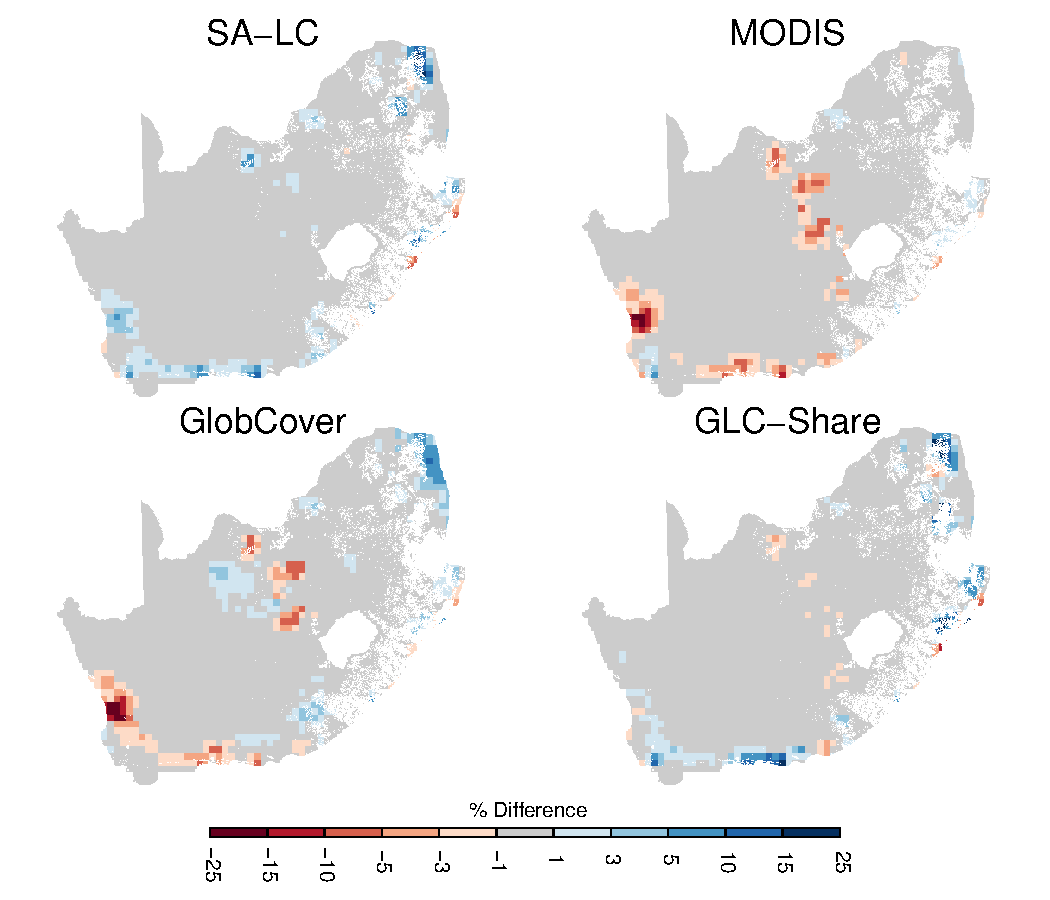
\includegraphics[width=.5\textwidth]{figures/et_bias_map.pdf}}
\caption{Differences in annual mean evapotranspiration estimates from 29-year runs of the VIC land surface hydrology model when initialized with LAI response curves derived from the reference map, versus those from the four cropland maps.}\label{afoto}
\end{figure}

\subsection{Initializing an agent-based model}
Spatially-explicit agent-based model (ABMs) are frequently employed to understand land use decision-making, often to facilitate improved policy, particularly in the arena of human development \cite{berger_creating_2006}. A common feature of such ABMs is that they need to be calibrated against data describing the characteristics of land users, including an initialization step to assign land resources to ``agents'' representing the land users, wherein the simulated landscape pattern and distribution of agent resources matches those in the real world. In our example, we used an ABM of household food security that simulate the interactions between many individual farming households (the agents) and their environment over multiple seasons \cite{chen_dependency_2013}. We used cropland maps to provide the model the location and abundance of cropland, which is used to allocate an initial share of cropland to each simulated household. Like many spatial ABMs, the model is computationally intensive, and thus run over smaller geographic domains (e.g. districts, rather than an entire country) and at higher spatial resolutions (10s to 100s of meters) in order to represent the different land units of single farmers. To match these computational characteristics, we selected four contiguous magisterial districts (ranging from 1,040-1,343 km$^2$, Fig. S8) in the eastern part of the country with 28-45\% of their areas devoted to cropland. The initialization process iteratively assigns households to the landscape using a function that factors in neighbor and cropland proximity, to ensure that households are grouped into communities and that their fields are within a realistic proximity. The number of households and the cropland area per household is derived from survey data of communities where all cropland is owned. The model is thus considered adequately initialized when all households are allocated their appropriate area of cropland, and all cropland is occupied. 

We used the reference map and each cropland map to separately initialize the model, and compared the agent allocation results to assess how cropland map errors impacted the initialization process. We examined three variable, the first being the number of agents that were not assigned fields, the second the amount of cropland left unallocated, and the third the area of land deficit, or the amount of land that should have been assigned to households but wasn't. For the first variable, there was a one-to-one relationship between the percentages by which cropland was underestimated and households that could not be assigned fields (Fig. 6, left panel). The most extreme examples occurred when MODIS cropland initialized the ABM in districts 1 and 2, where $\sim$85\% of agents did not receive cropland. All households were assigned fields when total cropland area was overestimated (GeoWiki, SA-LC), but in these cases the area of cropland allocated to no one (the second variable) was proportional to the size of the overestimate (e.g. $\sim$20\% for SA-LC, Fig. 6 right panel). Interestingly, the overall relationship between the percent of cropland allocated and percent cropland error was U-shaped, as the model also failed to give land to households when cropland was underestimated by more than 50\% (Fig. 6, right panel). MODIS again provided the most pronounced results in districts 1 and 2, where 7-12\% of cropland was left unallocated despite the fact that 85\% of agents had no land. This curious relationship occurred because cropland tends to cluster, and when it is underestimated, the size of these clusters is small, resulting in islands of cropland that fall outside of the search radius (which is constrained by an absolute distance and the proximity of other agents) within which cropland is sought when agents are seeded onto the landscape. 

The last measure, land deficit, increased exponentially in relation to cropland underestimation--reaching around 800\% for MODIS in districts 1 and 2--and would become infinite in the case of a 100\% underestimate.

%randomly siting 100 household agents within each district, and allocating the nearest two cropland pixels to each household. The remaining agents are then iteratively assigned unallocated cropland pixels within a 1.5 km radius of existing agents' fields, and this process continues until all agents are assigned cropland, or all available cropland is allocated. This initialization process 
%\FloatBarrier

\begin{figure}[!ht]
\centerline{\includegraphics[width=.5\textwidth]{figures/agent-bias.pdf}}
\caption{Biases in agent-based model initialization relative to the district-wise errors (as a percent) in total cropland area, measured in terms of the percent of households having no cropland allocated (left), and the percent of cropland left unallocated (right). Dot sizes correspond to district numbers, colors represent the landcover map.}
\label{afoto}
\end{figure}

\section{Discussion}
This spatially comprehensive, bottom-up assessment of landcover map bias and inaccuracy and provides unique insight into their extent, causes, and consequences for understanding global change processes, made possible by a unique, high accuracy dataset that likely provides the truest measure of total cropland area and distribution that is currently available for this region. This dataset is of course not perfect, being affected by the map-makers' occasional interpretation errors (mostly of omission), while some of the cropland map error we found may have been caused by the slight temporal mismatches between the reference data and the original landcover datasets we used. However, our assessment (SI) suggests that these errors are small, and do not appreciably impact our findings, which is bolstered by previous work showing the large scale of disagreements between landcover map-based cropland area estimates and national inventory data \cite{fritz_comparison_2010}.

Our results suggest several guidelines for using landcover data in global change research, and contain some important implications for how understanding of global change processes based on the data, and associated policy decisions, may be affected. In terms of developing a base landcover map, the first rule of thumb is that standard landcover products derived from coarse resolution sensors, such as MODIS and GlobCover, appear to be too biased to be useful without substantial aggregation. If we use the standard that bias within +/-10\% is acceptable, then at least 25-100 km of aggregation is needed to sufficiently cancel out the errors in the base landcover data and subsequent first order estimates built on them (Fig. 3 \& 4). The upper range of aggregation scale is necessary if a mixed pixel class becomes dominant, as in the case with GlobCover, because these lead to underestimation bias that will persist until the pixel size becomes substantially greater than the average area of landscapes that are dominated by the cover type of interest, which can be $>$1000 km$^2$ in some of South Africa's farming regions. 

Maps derived from higher resolution sensors, such as the SA-LC dataset, if carefully done, do not have this mixed class problem, and are sufficiently unbiased for most applications with just 1-5 km of aggregation. However, such datasets are typically developed for specific countries, using varying methods, and can be hard to obtain. For broader scale analyses, the best option is to use newer generation maps such as GeoWiki (and the GLC-Share \footnote{GLC-Share. www.glcn.org} datasets for other cover types) which is relatively unbiased at 1 km resolution. GeoWiki's lower bias comes from its process of evaluating consensus between several landcover datasets (including the other three in this study), resulting in cropland probabilities that are converted to percentages by calibrating to statistical data \cite{fritz_cropland_2011,fritz_mapping_2015}. This method mirrors the ensemble averaging used by other fields (e.g. crop \cite{asseng_uncertainty_2013}, climate \cite{giorgi_calculation_2002}, and ecological modeling \cite{araujo_ensemble_2007}) to increase prediction confidence. 

GeoWiki's statistical constraint procedure is similar to the one we used \cite[following][]{ramankutty_farming_2008}, which produced unbiased maize production estimates (Fig. 3) by eliminating bias in the adjusted cropland and harvested area maps that they were built upon. This result, together with GeoWiki's low bias, indicate the value of fusing inventory data with remote sensing. However, this method depends on the quality of inventory data, which are often suspect, particularly in Africa \cite{carletto_emperor_2013,fao_action_2013}. The statistical constraint also does not greatly improve map \emph{accuracy}, as evidenced by GeoWiki's 23\% mean absolute error in 1 km cropland percentage estimates (Fig. S1), which is only slightly more accurate than MODIS (31\%) but worse than SA-LC (11\%). GeoWiki is definitely most accurate among the large scale landcover products, but its improvement is related to the map consensus methods, which can correct for omission or commission errors made by the classifier. Statistical constraints only adjust map values at locations where cropland is identified, so their use it . 

Map accuracy is perhaps more important than bias for landcover maps.   



 
Broader regional implications - error higher elsewhere

Main points: 


What we found, significance of study 
\begin{itemize}
  \item First large area quantification of spatial biases
  \item How large those biases are, for one of the most widely spread (spreading landcovers)
  \item Insight into causes of bias, and thus some understanding of where biases are likely to be greater or smaller
  \item How much progress made in reducing it
  \item Class type and bias
\end{itemize}

\begin{itemize}
  \item Bias decreases as function of scale
  \item General bias patterns, appropriate use of landcover products, which landcover products
  \item Appropriate scales of inference, by type of product - 
  \item Aggregation improves results for landcover, generally, 
  \item Sensor resolution, statistical resolution, and merging products have high value
   \begin{itemize}
     \item But don't remove spatial bias - absolute bias matters. Statistical constraints seems to just compress spatial biases to higher rates of turnover. Geo-wiki
     \item But of course these types of data are then dependent on how accurate the statistical data are defining the constraint (cite emperor has no data)
    \end{itemize}
   \item Mixed landscapes increase the chances of omission and commission errors by increasing the number of cover classes, or because such landscapes are less spectrally distinct \cite{estes_diylandcover:_2015}
   \item caveats: Only single country in South Africa. More commercial farming than many other countries, but results are still instructive. Analysis of error as function of landscape type suggests that areas where cropland is more mixed with natural vegetation have higher errors. These sorts of landscapes quite common in smallholder-dominated systems, thus suggests that biases may be even higher elsewhere on the continent. 
\end{itemize}

Implications for understanding global change and policy: \\

Increasing awareness of need to have spatial assessments in global change analyses. Do things such as identify areas where yield gaps are high, or how much carbon or biodiversity will be lost to changes in land use, in order to try prioritize development \cite{searchinger_high_2015,newbold_global_2015}, or to understand coupled human-social dynamics, etc. \\

Our finding suggest:

\begin{itemize}
  \item Area-based estimates only safe at coarser scales of aggregation for most types of global change analyses, and primarily with constrained products. 
  \item 50-100 km scale of aggregation reduces bias sufficiently.
  \item Not so with unconstrained products
  \item Assessments of spatial variability unsafe, for all products, bar one - finer country-scale product.  Here you look at absolute bias. This is high in many products even at higher scales of aggregation. 
  \item This suggests that disaggregation approaches or paint by numbers approaches are nice maps, but can't give clear guidance about differences between grid cells, even when highly aggregated.  [work on this] 
  \item can lead to misinformed policies
  \begin{itemize}
    \item E.g. Efforts to identify area where yield gaps are most pronounced and/or concentrated are likely to be highly misleading, leading to ineffective targeting of resources. Most informative simply to look at these areas at the political boundary resolution
    \item Comparing carbon stocks against potential yield for tradeoff analysis, which may be done with conservation planning to find areas with high benefit/low-cost. Also misleading. 
    \item Looking at land availability for cropland or biofuels expansion (look at biofuel paper for example)--land might not be as available as people think. Can lead to formulation of bad policy
    \end{itemize}
  \item Analyses of higher order interactions, biogeochemistry, human decision-making, also misleading (maybe pair this with yield example). 
  \begin{itemize}
     \item Our example here, ET estimates not heavily biased, but in marginal areas of low rainfall some pronounced differences. These are areas where irrigation is more common, but VIC doesn't simulate this, so absolute bias in those zones likely to be underestimated, and such regions can have substantial impacts on altering climate \cite{estes_changing_2014, sacks_effects_2008}. 
    \item Can skew understanding of more advanced attempts to understand the human factors that go into driving agricultural productivity. Examples here
    \end{itemize}
\end{itemize}


Way forward
\begin{itemize}
  \item For now, use latest generation products fusion products or more detailed country-level products
  \item Avoid change detection based on landcover products, e.g. MODIS. 
  \item But moving forward key will be developing new approaches to map landcover with much greater fidelity, e.g. scaling out approach that led to this dataset, combining with latest computer vision algorithms, etc.  
\end{itemize} 




%Some points from my notes last year: 
%\begin{itemize}
%  \item Bias as a function of scale
%  \item Bias as a function of cropland cover
%    \begin{enumerate}
%      \item Classification algorithms are thus more error-prone where landcover is mixed/heterogenous.
%      \item The exception to this lies in the GlobCover dataset, where bias primarily increases as a function of cropland cover. The reason for this is that GlobCover's cropland classes do not provide for 100\% cropland cover, so aggregation tends to exacerbate underestimates. 
%      \item Thus caution is needed when aggregating a mixed pixel class.  
%        \begin{itemize} 
%          \item An example illustrates this: take 4 1 km pixels, 2 of which are 100\% cropland, 2 of which are other cover types. Imagine a landcover product classifies 3 of these as cropland (2 correct, 1 an error of commission), using a cropland class that is defined as 50\% cropland. Aggregating the actual fraction by a factor of 4 will result in a new 4 km pixel having 50\% cropland, whereas aggregating the landcover product's pixels will give just 38\% cropland, even when factoring in the incorrect classification.)
%          \end{itemize}
%    \end{enumerate}
%  \item Bias as a function of method
%      \begin{enumerate}
%        \item Higher resolution and ensemble-based approaches have less bias.
%        \item geowiki represents a fusion of multiple coarse resolution data sources that has undergone extensive validation using a crowdsourcing approach
%        \item the SALC dataset is based on 30 m landsat data, but incorporates a range of ancillary data and expert judgement
%        \item MODIS and GlobCover data are effectively single source/single algorithm.
%        \item \textbf{Newer points begin here}
%        \item Statistically constrained constrained landcover estimation approaches provide accurate area-based inferences when aggregated. But spatial errors are still high, as seen with GeoWiki and production/yield estimates. Using these to identify yield gaps at specific map locations is inappropriate, or even for a larger location if it does not coincide with the geographic boundaries of the statistical unit.  
%        \item Constrained estimates are also dependent on the accuracy of the statistics.  
%    \end{enumerate}
%  \item Fix above to have section on bias for global change studies
%    \begin{enumerate}
%      \item Scales at which it is safe to estimate values of say carbon stocks. 
%      \item Above point about bias in disaggregated yield estimates - no point mapping these out. A new approach might be to take these statistically reported yields and then combine them with satellite data to estimate yield variability within the district.  That way would have meaningful reason for disaggregating yields, and would be pegged to real yield values, which would help minimize errors in remote sensing of yields. 
%      \item Something on ET - doesn't seem to matter much, but land-atmosphere interactions can make these discrepancies meaningful, particularly since biases occur in arid areas where a lot of irrigation happens--can cause significant impacts on regional climate.  etc. etc. Also we didn't change out land cover types, and the vegetation in SA around the cropland will have reasonably similar LAI and ET responses (I think), thus impact more muted than it might be elsewhere (e.g. in forested landscapes).  
%      \item Agent-based models. \textcolor{red}{Tom, Peng, something of significance/implications of this, please}
%    \end{enumerate}
%  \item Will need a section on way forward for data, etc. Key role of accurate landcover, particularly agricultural.  New methods, vectorized field boundaries seem to be highly valuable, Mapping Africa, Stephanie's paper, Geo-Wiki, etc are the way ahead.  
%  
%    
%\end{itemize}


% $\theta$ changes from 0 to 1. (see Figure \ref{afoto}).That means we are considering $\theta$  of the form
%For these solutions we have the following

%\begin{remark}
%Note that equation \eqref{theta} specifies  the function $\varphi$
%up to an error of order $\delta$. Theorem 1 provides an evolution
%equation for the function $\varphi$ up to an error of order
%$\delta |log \delta|$.
%\end{remark}

%(see \eqref{weaksol}). 


\begin{materials}
\section{Methods} 
Perhaps it is right {\it SI Materials and Methods}.

Describe weighted mean bias reasons. 

We disaggregated the cropland percentages in all maps to binary cropland/non-cropland cover types with 100 m resolution, which matches the typical field size (1 ha) for smallholder farmers in household survey data (collected in Zambia) used in developing the agent-based model \cite{chen_dependency_2013}. The surveys provided the mean cropland area per household (2.2 ha) and frequencies distribution of cropland area holdings across households (e.g. how many households have 1 ha, 2 ha, etc.). We used these statistics to calculate the ``true'' number of households per district by dividing reference cropland areas by the mean cropland area, and preserved the cropland area distributions by multiplying the total number of households by the frequencies. We then initialized the model, which takes a weighted (by cropland area frequency) random draw of 100 households and places these within the district, assigning each household its required number of ``fields'' (cropland pixels), which must be within 1.5 km of the household's location and not already assigned to another household. This process is iterated until all households are assigned cropland, or all available cropland is allocated. 


\section{Digital RCD Analysis} 

\end{materials}

\appendix[App 1]

\appendix
This is an example of an appendix without a title.

\begin{acknowledgments}
I thank everyone tearfully. 
\end{acknowledgments}


% bib solution from here
% http://tex.stackexchange.com/questions/167650/is-there-a-more-recent-bibliography-style-file-bst-for-pnas
% https://github.com/jburon/pnas2011.bst
\bibliographystyle{pnas2011} 
{\footnotesize \bibliography{bias}}

%\begin{thebibliography}{10}
%\bibitem{BN}
%M.~Belkin and P.~Niyogi, {\em Using manifold structure for partially
%  labelled classification}, Advances in NIPS, 15 (2003).
%
%\bibitem{BBG:EmbeddingRiemannianManifoldHeatKernel}
%P.~B\'erard, G.~Besson, and S.~Gallot, {\em Embedding {R}iemannian
%  manifolds by their heat kernel}, Geom. and Fun. Anal., 4 (1994),
%  pp.~374--398.
%\end{thebibliography}


\end{article}

%\begin{figure}
%\centerline{\includegraphics[width=.4\textwidth]{figsamp.eps}}
%\caption{LKB1 phosphorylates Thr-172 of AMPK$\alpha$ \textit{in vitro}
%and activates its kinase activity.}\label{afoto}
%\end{figure}
%
%\begin{figure*}[ht]
%\begin{center}
%\centerline{\includegraphics[width=.7\textwidth]{figsamp.eps}}
%\caption{LKB1 phosphorylates Thr-172 of AMPK$\alpha$ \textit{in vitro}
%and activates its kinase activity.}\label{afoto2}
%\end{center}
%\end{figure*}
%
%\begin{table}[h]
%\caption{Repeat length of longer allele by age of onset class.
%This is what happens when the text continues.}
%\begin{tabular}{@{\vrule height 10.5pt depth4pt  width0pt}lrcccc}
%&\multicolumn5c{Repeat length}\\
%\noalign{\vskip-11pt}
%Age of onset,\\
%\cline{2-6}
%\vrule depth 6pt width 0pt years&\multicolumn1c{\it n}&Mean&SD&Range&Median\\
%\hline
%Juvenile, 2$-$20&40&60.15& 9.32&43$-$86&60\\
%Typical, 21$-$50&377&45.72&2.97&40$-$58&45\\
%Late, $>$50&26&41.85&1.56&40$-$45&42\tablenote{The no. of wells for all samples was 384. Genotypes were
%determined by mass spectrometric assay. The $m_t$ value indicates the
%average number of wells positive for the over represented allele.}
%\\
%\hline
%\end{tabular}
%\end{table}
%
%
%\begin{table*}[ht]
%\caption{Summary of the experimental results}
%\begin{tabular*}{\hsize}
%{@{\extracolsep{\fill}}rrrrrrrrrrrrr}
%\multicolumn{3}{l}{Parameters}&
%\multicolumn{5}{c}{Averaged Results}&
%\multicolumn{5}{c}{Comparisons}\cr
%\hline
%\multicolumn1c{$n$}&\multicolumn1c{$S^*_{MAX}$}&
%\multicolumn1c{$t_1$}&\multicolumn1c{\ $r_1$}&
%\multicolumn1c{\ $m_1$}&\multicolumn1c{$t_2$}&
%\multicolumn1c{$r_2$}&\multicolumn1c{$m_2$}
%&\multicolumn1c{$t_{lb}$}&\multicolumn1c{\ \ $t_1/t_2$}&
%$r_1/r_2$&$m_1/m_2$&
%$t_1/t_{lb}$\cr
%\hline
%10\tablenote{Stanford Synchrotron Radiation Laboratory (Stanford University,
%Stanford, CA)}&1\quad &4&.0007&4&4&.0020&4&4&1.000&.333&1.000&1.000\cr
%10\tablenote{$R_{\rm FREE}=R$ factor for the $\sim 5$\% of the randomly
%chosen unique ref\/lections not used in the ref\/inement.}&5\quad &50&.0008&8&50&.0020&12&49&.999&.417&.698&1.020\cr
%100\tablenote{Calculated for all observed data}&20\quad &2840975&.0423&95&2871117&.1083&521&---&
%.990&.390&.182&---\ \ \cr
%\hline
%\end{tabular*}
%\end{table*}


\end{document}


